\documentclass[12pt]{article}
\usepackage{amsmath, amssymb}
\usepackage{geometry}
\usepackage{amsfonts}
\usepackage{graphicx}
\geometry{margin=1in}

\title{Replication of\\\textit{Valuing Private Equity Investments Strip by Strip} by A. Gupta and S. Van Nieuwerburgh}
\author{Leonardo Cruciani}
\date{\today}

\begin{document}
\maketitle

\section{Introduction}\label{sec:introduction}
This document explains the replication of (part of) the paper \textit{Valuing Private Equity Investments Strip by Strip}, by Arpit Gupta and Stijn Van Nieuwerburgh.
The paper introduces a new method to value private equity (PE) investments by constructing replicating portfolios of publicly traded securities, namely zero-coupon bonds and equity strips.
A schematic overview of the paper is as follows:
\begin{itemize}
    \item They define the risk factor payoff time series, or \textit{strips}, and their corresponding prices, obtained through an asset pricing model.
    These risk factors are zero-coupon bonds, public equity dividends, public equity capital gains, etc.
    \item They regress the PE cash flows on the strips, and obtain the exposures using an elastic net.
    \item For each PE fund, they build a replicating portfolio on the public assets, with weights defined by the exposures and the asset prices.
    Thus, they identify two sources of time variation in PE funds expected returns (over the fund life): variation in the public asset returns and variation in exposures.
    \item They define the \texit{maturity} of the fund, which is then used to obtain the annualized expected fund returns.
    \item They define the net present value (NPV) of the fund as the sum of all risk-free rate-discounted future cash-flows minus the capital committed.
    \item They define the risk-adjusted profit (RAP) of the fund as the difference between the NPV of the actual PE fund and the NPV of the replicating portfolio.
    The outperformance in RAP is interpreted into an idiosyncratic component (i.e.\ funds that select the right portfolio of assets) and the reward for PE funds which can deliver exposure to risk factors at an after-fee cost that is lower than public markets.
    \item The null hypothesis is no outperformance, so zero expected RAP over all funds and horizons.
\end{itemize}
In the replication I will focus on the estimation of exposures.
In particular, I will use the asset pricing model code provided by the authors to obtain the strips, and write my own elastic net for the estimation of exposures.
Note that to obtain the strips, only publicly available data is required, while, the data for the PE cash-flows and other fund metadata is proprietary, and obtained from Preqin, as the author do.

\section{Construction of the strips}\label{sec:construction-of-the-strips}
The paper considers a total of $K=15$ risk factor payoff strips, as follows:
    \begin{itemize}
        \item 1 zero-coupon bond payoff strip
        \item 7 dividend strips on aggregate and factor-sorted portfolios
        \item 7 capital gain strips on aggregate and factor-sorted portfolios
    \end{itemize}
    In particular, the 7 strips for both the dividend and the capital gain strips are:
    \begin{itemize}
        \item Market (ME) – aggregate stock market
        \item Small stocks
        \item Large stocks
        \item Value stocks
        \item Growth stocks
        \item Real estate investment trusts (REITs)
        \item Infrastructure
    \end{itemize}
    Let $F_{t,t+h}$ denote the $K \times 1$ vector of risk factor payoffs over horizon $h$.
    Each element of $F_{t,t+h}$ corresponds to a specific strip:
    \begin{equation}
        F_{t,t+h} = \begin{bmatrix}
                        1 \\
                        \frac{D^m_{t+h}}{D^m_t} \\
                        \frac{P^m_{t+h}}{P^m_t} \\
                        \vdots \\
                        \frac{D^f_{t+h}}{D^f_t} \\
                        \frac{P^f_{t+h}}{P^f_t}
                    \end{bmatrix}
        \label{eq:risk_factors}
    \end{equation}
    Note the payoff of the zero-coupon bond bought at $t$ that matures at $t+h$ is simply 1.

\section{Estimating exposures}\label{sec:estimating-exposures}
    The authors introduce the following model:
    \begin{equation}
        X_{t+h}^i = \beta^i_{t,h} F_{t,t+h} +e^i_{t+h}
        \label{eq:exposures}
    \end{equation}
    where:
    \begin{itemize}
        \item $X_{t+h}^i$ is the net-of-fee cash-flow distribution for fund $i$ at $h=1,\hdots, 64$ quarters after its inception, $t$ (referred as \textit{vintage} of the fund).
        \item $F_{t,t+h}$ is the cash-flow strip vector from quarter $t$ to $t+h$, spanning years from 1974 to 2019, again with a $H=64$ quarters window.
        \item $\beta^i_{t,h}$ is the vector of exposures of fund $i$ to the cash-flow strips, at quarter $h$ since its vintage $t$.
        \item $e^i_{t+h}$ is the idiosyncratic cash-flow component, i.e., the residual.
    \end{itemize}
    They then proceed to estimate it using an elastic net:
    \begin{equation}
        \hat \beta = \arg \min _{\beta \in \mathbb R^{KH}_+} \left \Vert X_{t+h}^i - \beta_{t,h} F_{t,t+h} \right \Vert_2^2 + \lambda \left[(1-\alpha)\Vert \beta \Vert_2^2 + \alpha \Vert \beta \Vert_1\right]
        \label{eq:elastic-net}
    \end{equation}
    where $\lambda$ is the total penalty amount, and $\alpha$ the mixing parameter between LASSO ($\alpha =1$) and RIDGE ($\alpha =0$) penalties.
    Note that the estimation is restricted to only positive parameters.

    \subsection{Implementation}\label{subsec:implementation}
    In my implementation the regressions are run jointly for all 15 stips and 64 quarters of activity.
    Therefore, $KH=960$ parameters are estimated.
    The data is organized as follows:
    \begin{itemize}
        \item $F_{ikh}$ is a 3-dimensional tensor with dimensions $n_{funds} \times K \times H$, i.e., for each fund, we have a panel covering the realization of the 15 strips across 64 quarters, from inception to termination. Specifically, $h$ refers to the realization of the strip between the time of inception of the fund and the $h$-th quarter following the inception.
        \item $X_{ih}$ is a 2-dimensional tensor with dimensions $n_{funds} \times H$, i.e., for each fund, we have its cashflows across the 64 quarters of activity.
        \item $\beta_{kh}$ is a 2-dimensional tensor with dimensions $K \times H$, i.e., our aim is to estimate a cross-section of the average exposures to the different strips across 64 quarters of activity.
    \end{itemize}
    For the few funds lasting more than 16 years, all cashflows exceeding the last quarter are discounted split between the last 3 quarters, as the authors do in the paper.
    Thus, the model actually implemented is:
    \begin{equation}
        \hat X_{i,h} = \sum_{k=1}^K \beta_{kh} F_{ikh} , \qquad h=1,\hdots, H, \quad i = 1, \hdots, n_{funds}
    \end{equation}
    Before regressing, the funds are classified based on their asset class, according to fund metadata, and run separately.
    Three main asset classes are considered:
    \begin{itemize}
        \item Private Equity, referred in the paper as \textit{Buyout}, while the use Private Equity as an umbrella term.
        This asset class corresponds to what is usually called Private Equity.
        \item Venture Capital
        \item Real Estate
    \end{itemize}
    The optimal values for $\alpha$ and $\lambda$ are obtained trough a $5$-fold cross validation.

    \subsection{Results}\label{subsec:results}
    \begin{figure}[h!]
        \label{fig:betas}
        \centering
        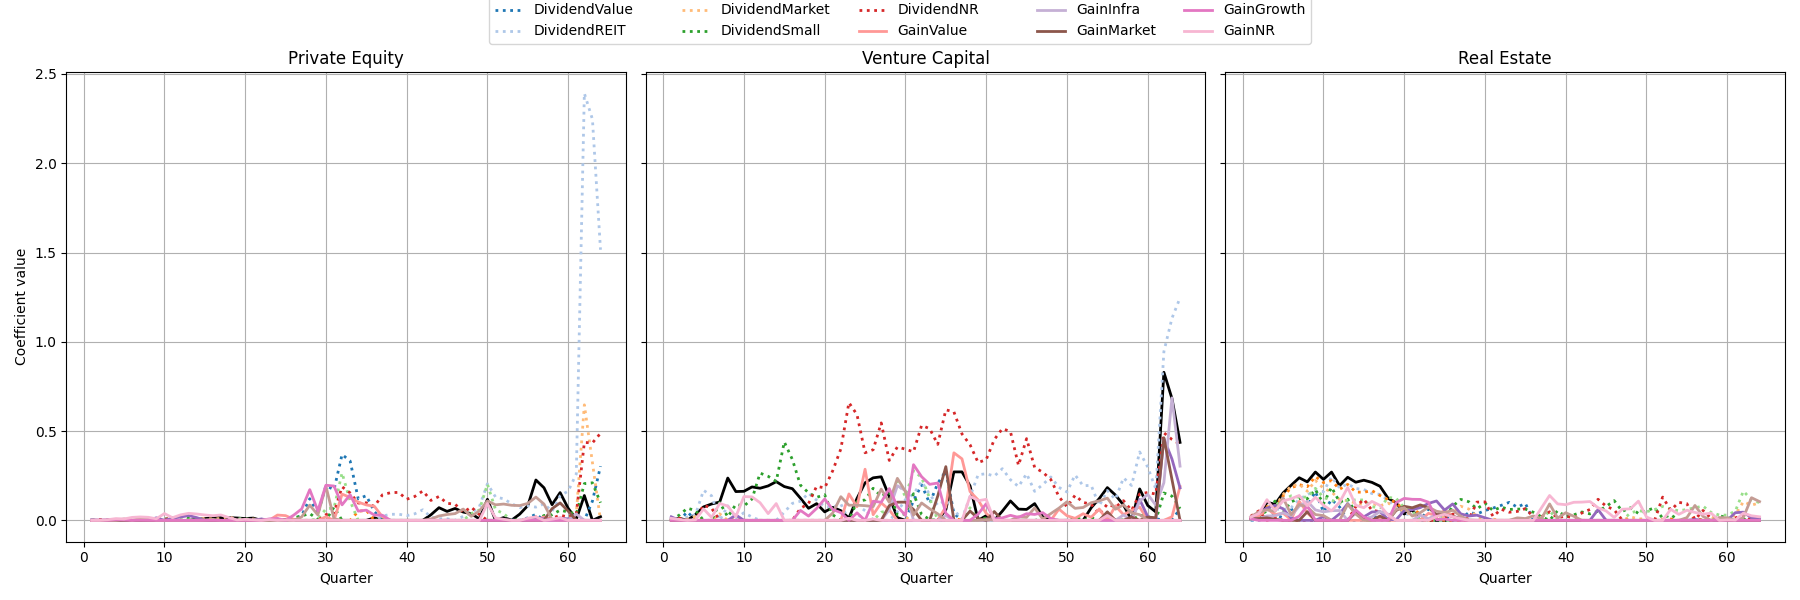
\includegraphics[width=0.9\linewidth]{img/img_1}
    \end{figure}

    \subsection{Code}
    The code consists of 6 parts, to be run after the execution of the code for strips generation provided by the authors, APmain.m:
    \begin{itemize}
        \item 01\_create\_strip\_data.py takes the output DividendStripOct20.Rda of APmain.m and organizes it in .csv file for further processing
        \item 02\_create\_pe\_cashflows.py takes the output DiscountRatesOct20.Rda of APmain.m, Preqin cashflow data and funds metadata, convert cashflow dates into quarters from inception (which comes from the metadata), scales cashflows to  and organizes it in .csv file for further processing

    \end{itemize}
\end{document}
